\documentclass{beamer}

\usepackage[francais]{babel}
\usepackage[T1]{fontenc}
\usepackage{amsmath}
\usepackage{color}
\usepackage{tikz}
\usepackage{graphicx}
\usepackage{algorithm2e}
\usepackage[adobe-utopia]{mathdesign}

\newcommand{\deriv}{\partial \!}

\usetikzlibrary{shapes,fit,calc,3d}

% Couleurs inspirées de famfamfam.com
\definecolor{vert}{HTML}{59FF2D}
\definecolor{bleu}{HTML}{0BCEFF}
\definecolor{rose}{HTML}{FF0B5B}
\definecolor{gris}{gray}{0.5}

\tikzset{line/.style={
    shorten >= -#1,
    shorten <= -#1}}
\tikzset{halfline/.style={
    shorten >= -#1}}
\tikzset{axe/.style={
    ->,
    thin}}
\tikzset{fig/.style={
    thick}}
\tikzset{origine/.style={
    draw=black,
    cross out}}
\tikzset{aabb/.style={
    dashed,
    thick,
    inner sep=0}}
\tikzset{gjknode/.style={
    fill=rose,
    circle}}
\tikzset{gjkedge/.style={
    draw=rose,
    thick}}
\tikzset{gjkdir/.style={
    halfline=0.5cm,
    draw=gris,
    very thick,
    dashed}}
\tikzset{gjkclosest/.style={
    circle,
    fill=bleu}}
\tikzset{rayon/.style={
    ->,
    dashed,
    draw=gris}}

\setbeamertemplate{headline}{
  \begin{beamercolorbox}[leftskip=5pt,ht=10pt]{section in head/foot}
    \insertsectionhead
  \end{beamercolorbox}
}
\setbeamertemplate{footline}[frame number]
\setbeamertemplate{navigation symbols}{}

% http://www.colourlovers.com/palette/694737/Thought_Provoking
\definecolor{brick}{HTML}{D95B43}
\definecolor{thoughtless}{HTML}{C02942}
\definecolor{thought}{HTML}{542427}
\definecolor{thoughtless2}{HTML}{53777A}

%\usecolortheme[named=tpe]{structure}
\setbeamercolor{title}{fg=brick}
\setbeamercolor{section in toc}{fg=thoughtless2}
\setbeamercolor{headline}{fg=thought}
\setbeamerfont{headline}{series=\small}
\setbeamercolor{frametitle}{fg=brick}
\setbeamerfont{frametitle}{series=\bfseries}
\setbeamercolor{item}{fg=thoughtless2}
\setbeamerfont{item title}{series=\bfseries}
\setbeamertemplate{itemize item}[square]

\title{Simulation physique de corps rigides avec interaction}
\author{Merwan Achibet\\ Université du Havre, 2011}
\date{}

\begin{document}

\shorthandoff{!} % Pour éviter bug de Tikz + Babel french

\AtBeginSection[]
{
  \thispagestyle{empty}
  \addtocounter{framenumber}{-1}
  \begin{frame}<beamer>{}
    \vspace{2.1em}
    \tableofcontents[currentsection]
  \end{frame}
}

\begin{frame}
  \thispagestyle{empty}
  \maketitle
\end{frame}

\begin{frame}{Table des matières}
  \thispagestyle{empty}
  \tableofcontents
\end{frame}

\setcounter{framenumber}{0}

\section{Introduction}

\begin{frame}{Moteur physique ?}
  Moteur physique : système de simulation mécanique
  \begin{description}
  \item[Industrie, science, cinéma] précis, lents
  \item[Jeu vidéo, réalité virtuelle] approximatifs, temps réel
  \end{description}

  \vfill
  
  Ce projet :
  \begin{itemize}
  \item Moteur physique de base 
  \item Corps rigides
  \item Corps convexes
  \item Temps réel
  \end{itemize}
\end{frame}

\begin{frame}{\'Etude de cas}
  \begin{enumerate}
  \item
    La chute

    \begin{align*}
      \vec{a} = \frac{1}{m} \sum_i \vec{F}_i
    \end{align*}
  \item
    Le rebond

    \begin{align*}
      &\vec{v}_1 = \gamma \vec{v}_2
    \end{align*}
  \item
    Le repos

    \begin{columns}
      \begin{column}{3cm}
        \[\vec{F}_{A/B} = -\vec{F}_{B/A}\]
      \end{column}
      \begin{column}{3cm}
        \[\vec{F}_{A/B} + \vec{F}_{B/A} = 0\]
      \end{column}
    \end{columns}
  \end{enumerate}
\end{frame}

\begin{frame}{Différentes tâches}
  \begin{itemize}
  \item Dynamique
    \begin{itemize}
    \item Composante linéaire
    \item Composante angulaire
    \end{itemize}

    \vfill

  \item Gestion des collisions
    \begin{itemize}
    \item Détection
    \item Correction
    \item Réponse
    \end{itemize}
  \end{itemize}
\end{frame}

\section{Dynamique}

\subsection{Composante linéaire}

\begin{frame}{La composante linéaire}
  \begin{description}
  \item[Entrée] Forces environnementales
  \item[Sortie] Changement de position
  \end{description}

  \vfill

  \begin{columns}
    \begin{column}{3cm}
      \begin{align*}
        \vec{v} &= \frac{\deriv \vec{p}}{\deriv t} \\ \\
        \vec{a} &= \frac{\deriv \vec{v}}{\deriv t}
      \end{align*}
    \end{column}
    \begin{column}{2cm}
      \centering
      $\iff$
    \end{column}
    \begin{column}{3cm}
      \begin{align*}
        \vec{p} = \int \vec{v}\; \deriv t \\ \\
        \vec{v} = \int \vec{a}\; \deriv t
      \end{align*}
    \end{column}
  \end{columns}
\end{frame}

\begin{frame}{Intégration de la composante linéaire}
  Intégration d'Euler :
  \begin{align*}
    x_{n+1} = x_{n} + x' \deriv t
  \end{align*}

  \vfill

  Appliquée à nos besoins :
  \begin{align*}
    \vec{a}_{t + \deriv t} &= \frac{1}{m} \sum_i \vec{F}_i \\ \\
    \vec{v}_{t + \deriv t} &= \vec{v}_t + \vec{a}_{t + \deriv t} \deriv t \\ \\
    \vec{p}_{t + \deriv t} &= \vec{p}_t + \vec{v}_{t + \deriv t} \deriv t
  \end{align*}
\end{frame}

\begin{frame}{Simplification grâce à l'élan linéaire}
  L'élan linéaire :
  \begin{columns}
    \begin{column}{3cm}
      \begin{align*}
        \vec{L} = m \vec{v}
      \end{align*}
    \end{column}
    \begin{column}{3cm}
      \begin{align*}
        \sum_i \vec{F}_i = \frac{\deriv \vec{L}}{\deriv t} = \frac{\deriv (m\vec{v})}{\deriv t}
      \end{align*}
    \end{column}
  \end{columns}

  \vfill

  La nouvelle intégration :
  \begin{align*}
    \vec{L}_{t + \deriv t} &= \vec{L}_t + {\sum_i \vec{F}_i} \\ \\
    \vec{p}_{t + \deriv t} &= \vec{p}_t + \frac{1}{m}\vec{L}_{t + \deriv t} \deriv t
  \end{align*}
\end{frame}

\begin{frame}{Modélisation d'un corps}
  OK pour une particule, mais un objet plus complexe ?
  \begin{description}
  \item[Une particule = un sommet] Non
  \item[Une unique particule judicieusement placée] Oui, le centre de masse
  \end{description}

  \vfill

  \begin{align*}
    \vec{C} = \frac{1}{M} \sum_i m_i \vec{p}_i
  \end{align*}
\end{frame}

\begin{frame}{Le centre de masse}
  Centre de masse = origine du repère local

  \vfill

  \begin{figure}
    \begin{tikzpicture}
  % repère
\draw[->] (-0.2,0) -- (10,0);
\draw[->] (0,-0.2) -- (0,10);
\foreach \i in {0,...,9}
{
  \draw[xshift=\i cm] (0,-1pt) -- (0,1pt);
  \draw[yshift=\i cm] (-1pt,0) -- (1pt,0);
}

  % figure
  \coordinate (C) at ++(6,5);
  \draw (C) circle (2);

  % repère local  
  \begin{scope}[rotate around={-30:(C)}]
    \draw[->] (C) -- +(4,0);
    \draw[->] (C) -- +(0,4);
  \end{scope}
\end{tikzpicture}

  \end{figure}

  \vfill

  \begin{align*}
    \vec{p}_l = \vec{p}_a - \vec{C}
  \end{align*}
\end{frame}

\subsection{Composante angulaire}

\begin{frame}{La composante angulaire}
  Il manque quelque chose... Les rotations !

  \begin{description}
  \item[Matrice d'orientation]
    Un vecteur colonne = un axe du repère local
    \begin{align*}
      \begin{pmatrix}
        1 & 0 & 0 \\ 0 & 1 & 0 \\ 0 & 0 & 1
      \end{pmatrix}
      \rightarrow
      \begin{pmatrix}
        1 \\ 0 \\ 0
      \end{pmatrix}
      \begin{pmatrix}
        0 \\ 1 \\ 0
      \end{pmatrix}
      \begin{pmatrix}
        0 \\ 0 \\ 1
      \end{pmatrix}
    \end{align*}
    
    \vfill

  \item[\'Elan angulaire]
    Analogue à l'élan linéaire
    \begin{columns}
      \begin{column}{3cm}
        \begin{align*}
          \vec{A}_{t + \deriv t} &= \vec{A}_n + {\sum_i \vec{\tau}_i}
        \end{align*}
      \end{column}
      \begin{column}{3cm}
        \begin{align*}
          \vec{\tau}_i &= (\vec{x} - \vec{C}) \times \vec{F}_i
        \end{align*}
      \end{column}
    \end{columns}
  \end{description}
\end{frame}

\begin{frame}{Quantités auxiliaires I}
  Passage de l'élan à la nouvelle orientation moins direct.
  
  \vfill

  \begin{description}
  \item[Tenseur d'inertie local]
    Matrice représentant les efforts à fournir pour produire une rotation le long de chaque axe

    \vfill

  \item[Tenseur d'inertie absolu]
    Pendant absolu du tenseur d'inertie local
    \begin{align*}
      I_a = R I_l {}^t\!\!R
    \end{align*}

    \vfill

  \item[Vitesse angulaire]
    \begin{align*}
      \vec{\omega} = I^{-1}_a \vec{A}
    \end{align*}
  \end{description}
\end{frame}

\begin{frame}{Quantités auxiliaires II}
  On définit l'opérateur $*$ :

  \begin{align*}
    \begin{pmatrix}
      x \\ y \\ z
    \end{pmatrix}
    ^*
    =
    \begin{pmatrix}
      0 & -z & y \\ z & 0 & -x \\ -y & x & 0
    \end{pmatrix}
  \end{align*}
  
  \vfill

  On multiplie $\vec{\omega}$ et chaque axe de $R$ : 
  \begin{align*}
    \frac{\deriv R}{\deriv t} =
    \begin{pmatrix}
      \vec{\omega}^* \begin{pmatrix} R_{xx} \\ R_{xy} \\ R_{xz} \end{pmatrix} & 
      \vec{\omega}^* \begin{pmatrix} R_{yx} \\ R_{yy} \\ R_{yz} \end{pmatrix} & 
      \vec{\omega}^* \begin{pmatrix} R_{zx} \\ R_{zy} \\ R_{zz} \end{pmatrix} \\
    \end{pmatrix}
  \end{align*}
    
  \vfill

  Soit :
  \begin{align*}
    \frac{\deriv R}{\deriv t} = \vec{\omega}^*R
  \end{align*}  
\end{frame}

\begin{frame}{Intégration de la composante angulaire}
  \begin{align*}
    \vec{A}_{t + \deriv t} &= \vec{A}_t + \sum_i \vec{\tau}_i \\ \\
    I_a &= R_t I_l {}^t\!\!R_t \\ \\
    \vec{\omega} &= I^{-1}_a \vec{A}_{t + \deriv t} \\ \\
    R_{t + \deriv t} &= R_t + \vec{\omega}^* R_t \deriv t
  \end{align*}
\end{frame}

\section{Collisions}

\subsection{Détection}

\begin{frame}{Deux niveaux de précision}
  On teste les collisions entre paires de corps : $\frac{n(n-1)}{2}$ tests

  \vfill

  Beaucoup de tests, on veut accélérer le processus.

  \vfill

  \begin{description}
  \item[1. Détection grossière] \'Economique, faux positif possible 
  \item[2. Détection fine] Précise, plus coûteuse
  \end{description}
\end{frame}

\begin{frame}{Détection grossière}
  \begin{overprint}

    \onslide<1>
    \begin{figure}
      \centering
      \begin{tikzpicture}[scale=0.7, transform shape]
  % repère
\draw[->] (-0.2,0) -- (10,0);
\draw[->] (0,-0.2) -- (0,10);
\foreach \i in {0,...,9}
{
  \draw[xshift=\i cm] (0,-1pt) -- (0,1pt);
  \draw[yshift=\i cm] (-1pt,0) -- (1pt,0);
}

  \coordinate (R) at (7,3);
  \node[rectangle,rotate=-30,minimum height=3cm, minimum width=2cm,inner sep=0pt,draw=black] (rect) at (R) {};
  \coordinate (C) at (2,7);
  \node[circle,minimum size=2cm,inner sep=0pt,draw=black] (cerc) at (C) {};

  \begin{scope}[rotate around={-30:(C)}]
    \path (R) node () {}
          ++(-1,-1.5) node (a) {}
          ++(2,0) node (b) {}
          ++(0,3) node (c) {}
          ++(-2,0) node (d) {};
   \end{scope}

  % bounding boxes
  \node[fit=(a) (b) (c) (d),draw=green,dashed] {};
  \node[fit=(cerc),draw=green,dashed] {};

\end{tikzpicture}

    \end{figure}
    \begin{description}
    \item[Boîte englobante] Contient tous les sommets, donc tous les points
    \item[SAT] Test rapide de collision entre boîtes
    \end{description}

    \onslide<2>
    \begin{figure}
      \centering
      \begin{tikzpicture}[scale=0.7, transform shape]
  % repère
\draw[->] (-0.2,0) -- (10,0);
\draw[->] (0,-0.2) -- (0,10);
\foreach \i in {0,...,9}
{
  \draw[xshift=\i cm] (0,-1pt) -- (0,1pt);
  \draw[yshift=\i cm] (-1pt,0) -- (1pt,0);
}

  \coordinate (R) at (7,3);
  \node[rectangle,rotate=-30,minimum height=3cm, minimum width=2cm,inner sep=0pt,draw=black] (rect) at (R) {};
  \coordinate (C) at (2,7);
  \node[circle,minimum size=2cm,inner sep=0pt,draw=black] (cerc) at (C) {};

  \begin{scope}[rotate around={-30:(C)}]
    \path (R) node () {}
          ++(-1,-1.5) node (a) {}
          ++(2,0) node (b) {}
          ++(0,3) node (c) {}
          ++(-2,0) node (d) {};
   \end{scope}

  % bounding boxes
  \node[fit=(a) (b) (c) (d),draw=green,dashed] {};
  \node[fit=(cerc),draw=green,dashed] {};

\end{tikzpicture}

    \end{figure}
    \begin{description}
    \item[Faux positif] La détection fine invalidera le résultat
    \end{description}

    \onslide<3>
    \begin{figure}
      \centering
      \begin{tikzpicture}[scale=0.7, transform shape]
  % repère
\draw[->] (-0.2,0) -- (10,0);
\draw[->] (0,-0.2) -- (0,10);
\foreach \i in {0,...,9}
{
  \draw[xshift=\i cm] (0,-1pt) -- (0,1pt);
  \draw[yshift=\i cm] (-1pt,0) -- (1pt,0);
}

  \coordinate (R) at (7,3);
  \node[rectangle,rotate=-30,minimum height=3cm, minimum width=2cm,inner sep=0pt,draw=black] (rect) at (R) {};
  \coordinate (C) at (2,7);
  \node[circle,minimum size=2cm,inner sep=0pt,draw=black] (cerc) at (C) {};

  \begin{scope}[rotate around={-30:(C)}]
    \path (R) node () {}
          ++(-1,-1.5) node (a) {}
          ++(2,0) node (b) {}
          ++(0,3) node (c) {}
          ++(-2,0) node (d) {};
   \end{scope}

  % bounding boxes
  \node[fit=(a) (b) (c) (d),draw=green,dashed] {};
  \node[fit=(cerc),draw=green,dashed] {};

\end{tikzpicture}

    \end{figure}
    \begin{description}
    \item[Collision détectée] La détection fine validera le résultat
    \end{description}

  \end{overprint}
\end{frame}

\begin{frame}{Détection fine I}
  \begin{description}
  \item[Somme de Minkowski]
    $A \oplus B = \{a + b \mid a \in A, b \in B\}$
  \item[Différence de Minkowski]
    $A \ominus B = A \oplus (-B)$
  \end{description}

  \begin{figure}
    \centering
    \begin{tikzpicture}[scale=0.5,transform shape]
  \begin{scope}[scale=0.7]
    % repère
\draw[->] (-0.2,0) -- (10,0);
\draw[->] (0,-0.2) -- (0,10);
\foreach \i in {0,...,9}
{
  \draw[xshift=\i cm] (0,-1pt) -- (0,1pt);
  \draw[yshift=\i cm] (-1pt,0) -- (1pt,0);
}
  \end{scope}

  % Rectangle
\coordinate (a1) at (4,5);
\coordinate (a2) at (4,3);
\coordinate (a3) at (6,3);
\coordinate (a4) at (6,5);

% Triangle
\coordinate (b1) at (1,2);
\coordinate (b2) at (1,1);
\coordinate (b3) at (3,1);

% Minkowski difference
\coordinate (m1) at (1,4);
\coordinate (m2) at (1,2);
\coordinate (m3) at (3,1);
\coordinate (m4) at (5,1);
\coordinate (m5) at (5,4);


  \draw[black] (a1) -- (a2) -- (a3) -- (a4) -- cycle;
  \node[black] at (5,4) (a) {$A$};

  \draw[black] (b1) -- (b2)-- (b3) -- cycle;
  \node[black] at (1.5,1.5) (b) {$B$};

  \draw[<->,bleu,thick,dashed] (a2) -- ($(b1)!(a2)!(b3)$);
\end{tikzpicture}

    \begin{tikzpicture}[scale=0.55,transform shape]
  \begin{scope}[scale=0.7]
    % repère
\draw[->] (-0.2,0) -- (10,0);
\draw[->] (0,-0.2) -- (0,10);
\foreach \i in {0,...,9}
{
  \draw[xshift=\i cm] (0,-1pt) -- (0,1pt);
  \draw[yshift=\i cm] (-1pt,0) -- (1pt,0);
}
  \end{scope}

  % Rectangle
\coordinate (a1) at (4,5);
\coordinate (a2) at (4,3);
\coordinate (a3) at (6,3);
\coordinate (a4) at (6,5);

% Triangle
\coordinate (b1) at (1,2);
\coordinate (b2) at (1,1);
\coordinate (b3) at (3,1);

% Minkowski difference
\coordinate (m1) at (1,4);
\coordinate (m2) at (1,2);
\coordinate (m3) at (3,1);
\coordinate (m4) at (5,1);
\coordinate (m5) at (5,4);

  
  \draw[black,thick] (m1) -- (m2) -- (m3) -- (m4) -- (m5) -- cycle;
  \node[black] at (3,3) (m) {$A \ominus B$};

  \draw[<->,vert,thick, dashed] (0,0) -- ($(m2)!(0,0)!(m3)$);
\end{tikzpicture}

  \end{figure}

  \begin{description}
  \item[Particularité]
    La plus petite distance de la différence de Minkowski à l'origine est la plus petite distance entre les corps $A$ et $B$
  \end{description}
\end{frame}

\begin{frame}{Détection fine II}
  Comment calculer la plus petite distance entre $M$ et l'origine ?

  \vfill

  \begin{description}
  \item[Algorithme GJK]
    Expansion d'un simplex jusqu'à ce qu'il contienne le point le plus proche de l'origine.
  \end{description}

  \vfill

  \begin{description}
  \item[Simplex] Structure géométrique entièrement contenue dans $M$ et liée à une dimension.
    \begin{description}
    \item[0] Sommet
    \item[1] Arête
    \item[2] Triangle
    \item[3] Tétraèdre
    \end{description}
  \end{description}
\end{frame}

\begin{frame}{Détection fine III}
  Comment guider la recherche ?

  \vfill

  \begin{description}
    \item[$S(\vec{d})$]
      Fonction de support renvoyant le sommet de $M$ le plus extrême dans la direction $\vec{d}$

      \vfill

    \item[Avantage]
      $S_{A \ominus B}(\vec{d}) = S_A(\vec{d}) - S_B(-\vec{d})$ \\
      Inutile de calculer explicitement $M$ !
  \end{description}
\end{frame}

\begin{frame}{Détection fine IV}
  \begin{figure}
    \centering
    \begin{tikzpicture}[scale=0.7,transform shape]
	\coordinate (A) at (9,2);
\coordinate (B) at (4,1);
\coordinate (C) at (1,4);
\coordinate (D) at (2,7);
\coordinate (E) at (7,7);
\coordinate (O) at (2,2);

\node[origine] (origin) at (O) {};
\path[draw=black] (A) -- (B) -- (C) -- (D) -- (E) -- cycle;


	\node[draw=red, circle] (a) at (A) {};
  
\end{tikzpicture}

    \begin{tikzpicture}[scale=0.7,transform shape]
	\coordinate (A) at (9,2);
\coordinate (B) at (4,1);
\coordinate (C) at (1,4);
\coordinate (D) at (2,7);
\coordinate (E) at (7,7);
\coordinate (O) at (2,2);

\node[origine] (origin) at (O) {};
\path[draw=black] (A) -- (B) -- (C) -- (D) -- (E) -- cycle;


	\node[gjknode] (a) at (A) {};
	\node[gjknode] (c) at (C) {};
  
  \path[gjkpath] (a) -- (c);
\end{tikzpicture}

    \begin{tikzpicture}[scale=0.7,transform shape]
	\coordinate (A) at (9,2);
\coordinate (B) at (4,1);
\coordinate (C) at (1,4);
\coordinate (D) at (2,7);
\coordinate (E) at (7,7);
\coordinate (O) at (2,2);

\node[origine] (origin) at (O) {};
\path[draw=black] (A) -- (B) -- (C) -- (D) -- (E) -- cycle;


	\node[draw=red, circle] (a) at (A) {};
	\node[draw=red, circle] (c) at (C) {};
	\path[draw=green] (a) -- (c);
  
\end{tikzpicture}

    \begin{tikzpicture}[scale=0.4,transform shape]
	\coordinate (A) at (9,2);
\coordinate (B) at (4,1);
\coordinate (C) at (1,4);
\coordinate (D) at (2,7);
\coordinate (E) at (7,7);
\coordinate (O) at (2,2);

\node[origine] (origin) at (O) {};
\path[draw=black] (A) -- (B) -- (C) -- (D) -- (E) -- cycle;


	\node[gjknode] (a) at (A) {};
	\node[gjknode] (c) at (C) {};
	\node[gjknode] (b) at (B) {};

	\draw[gjkedge] (a) -- (c) -- (b) -- (a);
  \fill[rose,opacity=0.1] (A) -- (C) -- (B);

  \node[gjkclosest] (closest) at ($(C)!(O)!(B)$) {};
\end{tikzpicture}

    \begin{tikzpicture}[scale=0.4,transform shape]
	\coordinate (A) at (9,2);
\coordinate (B) at (4,1);
\coordinate (C) at (1,4);
\coordinate (D) at (2,7);
\coordinate (E) at (7,7);
\coordinate (O) at (2,2);

\node[origine] (origin) at (O) {};
\path[draw=black] (A) -- (B) -- (C) -- (D) -- (E) -- cycle;


	\node[gjknode] (c) at (C) {};
	\node[gjknode] (b) at (B) {};

	\path[gjkedge] (c) -- (b);
  
\end{tikzpicture}

    \begin{tikzpicture}[scale=0.4,transform shape]
	\coordinate (A) at (9,2);
\coordinate (B) at (4,1);
\coordinate (C) at (1,4);
\coordinate (D) at (2,7);
\coordinate (E) at (7,7);
\coordinate (O) at (2,2);

\node[origine] (origin) at (O) {};
\path[draw=black] (A) -- (B) -- (C) -- (D) -- (E) -- cycle;


  \node[gjkclosest] (closest) at ($(C)!(O)!(B)$) {};

  \node at ($(closest)+(0.4,0)$) (lclosest) {$S_2$};
\end{tikzpicture}

  \end{figure}
\end{frame}

\subsection{Correction}

\begin{frame}{Correction I}
  \begin{description}
  \item[Intégration d'Euler] Simulation discrète, pas de temps fixe
  \item[Problème] Les collisions sont toujours pénétrantes
  \end{description}

  \vfill

  \begin{figure}
    \centering
    \begin{tikzpicture}[scale=0.7, transform shape]

\coordinate (A1) at (0,0);
\coordinate (A2) at (6.7,0);
\coordinate (B) at (8,0);

\draw node[fig,
  circle,
  minimum size=2cm,
  draw=bleu,
  dotted] (a1) at (A1) {};

\node[fig,
  circle,
  minimum size=2cm,
  draw=bleu] (a2) at (A2) {};

\node[fig,
  circle,
  minimum size=2cm,
  draw=rose] (b) at (B) {};

\draw[->,thick,vert] (A1) to node[black,auto] {$+ \deriv t$} (A2);

\end{tikzpicture}

  \end{figure}

  \vfill

  \begin{description}
  \item[Solution] Intégrer en arrière, par dichotomie
  \end{description}
\end{frame}

\begin{frame}{Correction II}
  \begin{figure}
    \centering
    \begin{tikzpicture}[scale=0.7, transform shape]

\coordinate (A1) at (0,0);
\coordinate (B) at (8,0);

\coordinate (A2) at (6.7,0);
\coordinate (A2prec) at (A1);
\draw node[fig,
  circle,
  minimum size=2cm,
  draw=blue,
  dotted] (a1) at (A1) {};

\node[fig,
  circle,
  minimum size=2cm,
  draw=blue] (a2) at (A2) {};

\node[fig,
  circle,
  minimum size=2cm,
  draw=rose] (b) at (B) {};

\node[
  circle,
  dashed,
  minimum size=2.5cm,
  draw=rose] (btol) at (B) {};

\draw[->,thick,vert,font=\Large] (A2prec) to node[black,auto] {$+ \deriv t$} (A2);

\coordinate (A1) at ($(A1) + (0,-3)$);
\coordinate (A2) at ($(A2) + (0,-3)$);
\coordinate (A2prec) at ($(A2prec) + (0,-3)$);
\coordinate (B) at ($(B) + (0,-3)$);
\coordinate (A2precT) at (A2prec);
\coordinate (A2prec) at (A2);
\coordinate (A2) at ($(A2)!0.5!(A2precT)$);
\draw node[fig,
  circle,
  minimum size=2cm,
  draw=blue,
  dotted] (a1) at (A1) {};

\node[fig,
  circle,
  minimum size=2cm,
  draw=blue] (a2) at (A2) {};

\node[fig,
  circle,
  minimum size=2cm,
  draw=rose] (b) at (B) {};

\node[
  circle,
  dashed,
  minimum size=2.5cm,
  draw=rose] (btol) at (B) {};

\draw[->,thick,vert,font=\Large] (A2prec) to node[black,auto,swap] {$- \frac{\deriv t}{2}$} (A2);

\coordinate (A1) at ($(A1) + (0,-3)$);
\coordinate (A2) at ($(A2) + (0,-3)$);
\coordinate (A2prec) at ($(A2prec) + (0,-3)$);
\coordinate (B) at ($(B) + (0,-3)$);
\coordinate (A2precT) at (A2prec);
\coordinate (A2prec) at (A2);
\coordinate (A2) at ($(A2)!0.5!(A2precT)$);
\draw node[fig,
  circle,
  minimum size=2cm,
  draw=blue,
  dotted] (a1) at (A1) {};

\node[fig,
  circle,
  minimum size=2cm,
  draw=blue] (a2) at (A2) {};

\node[fig,
  circle,
  minimum size=2cm,
  draw=rose] (b) at (B) {};

\node[
  circle,
  dashed,
  minimum size=2.5cm,
  draw=rose] (btol) at (B) {};

\draw[->,thick,vert,font=\Large] (A2prec) to node[black,auto] {$+ \frac{\deriv t}{4}$} (A2);

\coordinate (A1) at ($(A1) + (0,-3)$);
\coordinate (A2) at ($(A2) + (0,-3)$);
\coordinate (A2prec) at ($(A2prec) + (0,-3)$);
\coordinate (B) at ($(B) + (0,-3)$);
\coordinate (A2precT) at (A2prec);
\coordinate (A2prec) at (A2);
\coordinate (A2) at ($(A2)!-1!(A2precT)$);
\draw node[fig,
  circle,
  minimum size=2cm,
  draw=blue,
  dotted] (a1) at (A1) {};

\node[fig,
  circle,
  minimum size=2cm,
  draw=blue] (a2) at (A2) {};

\node[fig,
  circle,
  minimum size=2cm,
  draw=rose] (b) at (B) {};

\node[
  circle,
  dashed,
  minimum size=2.5cm,
  draw=rose] (btol) at (B) {};

\draw[->,thick,vert,font=\Large] (A2prec) to node[black,auto] {$+ \frac{\deriv t}{4}$} (A2);

\coordinate (A1) at ($(A1) + (0,-3)$);
\coordinate (A2) at ($(A2) + (0,-3)$);
\coordinate (A2prec) at ($(A2prec) + (0,-3)$);
\coordinate (B) at ($(B) + (0,-3)$);
\coordinate (A2precT) at (A2prec);
\coordinate (A2prec) at (A2);
\coordinate (A2) at ($(A2)!0.5!(A2precT)$);
\draw node[fig,
  circle,
  minimum size=2cm,
  draw=blue,
  dotted] (a1) at (A1) {};

\node[fig,
  circle,
  minimum size=2cm,
  draw=blue] (a2) at (A2) {};

\node[fig,
  circle,
  minimum size=2cm,
  draw=rose] (b) at (B) {};

\node[
  circle,
  dashed,
  minimum size=2.5cm,
  draw=rose] (btol) at (B) {};

\draw[->,thick,vert,font=\Large] (A2prec) to node[black,auto,swap] {$- \frac{\deriv t}{8}$} (A2);

\end{tikzpicture}

  \end{figure}
\end{frame}

\subsection{Réponse}

\begin{frame}{Réponse I}
  \begin{description}
  \item[Corps rigide] Défini par sommets, arêtes et faces
  \end{description}
  
  \vfill

  On s'intéresse uniquement aux contacts sommet-face et arête-arête.

  \vfill

  \begin{figure}
    \centering
    \begin{tikzpicture}[scale=0.4]
  % Avant.
  \begin{scope}[canvas is xy plane at z=4]
    \path[fill=gris!20] (0,0) rectangle (4,4);
  \end{scope}
  % Droite.
  \begin{scope}[canvas is zy plane at x=4]
    \path[fill=gris!50] (0,0) rectangle (4,4);
  \end{scope}
  % Haut.
  \begin{scope}[canvas is zx plane at y=4]
    \path[fill=gris!70] (0,0) rectangle (4,4);
  \end{scope}

  % Avant.
  \begin{scope}[canvas is xy plane at z=2]
    \path[fill=gris!20] (2,4) rectangle (6,8);
  \end{scope}
  % Droite.
  \begin{scope}[canvas is yz plane at x=6]
    \path[fill=gris!50] (4,2) rectangle (8,-2);
  \end{scope}
  % Haut.
  \begin{scope}[canvas is xz plane at y=8]
    \path[fill=gris!70] (2,2) rectangle (6,-2);
  \end{scope}
\end{tikzpicture}

    w\begin{tikzpicture}[scale=0.4]
  % Avant.
  \begin{scope}[canvas is xy plane at z=4]
    \path[draw=black, thick] (0,0) rectangle (4,4);
  \end{scope}
  % Droite.
  \begin{scope}[canvas is zy plane at x=4]
    \path[draw=black, thick] (0,0) rectangle (4,4);
  \end{scope}
  % Arrière.
  \begin{scope}[canvas is xy plane at z=0]
    \path[draw=black,dashed,thin] (0,0) rectangle (4,4);
  \end{scope}
  % Gauche.
  \begin{scope}[canvas is yz plane at x=0]
    \path[draw=black,dashed,thin] (0,0) rectangle (4,4);
  \end{scope}
  % Haut.
  \begin{scope}[canvas is zx plane at y=4]
    \path[draw=black, thick] (0,0) rectangle (4,4);
  \end{scope}

  % Avant.
  \begin{scope}[canvas is xy plane at z=2]
    \path[draw=black, thick] (2,4) rectangle (6,8);
  \end{scope}
  % Droite.
  \begin{scope}[canvas is yz plane at x=6]
    \path[draw=black, thick] (4,2) rectangle (8,-2);
  \end{scope}
  % Haut.
  \begin{scope}[canvas is xz plane at y=8]
    \path[draw=black, thick] (2,2) rectangle (6,-2);
  \end{scope}
  % Arrière.
  \begin{scope}[canvas is xy plane at z=-2]
    \path[draw=black,dashed,thin] (2,4) rectangle (6,8);
  \end{scope}
  % Gauche.
  \begin{scope}[canvas is yz plane at x=2]
    \path[draw=black,dashed,thin] (4,2) rectangle (8,-2);
  \end{scope}

  \begin{scope}[canvas is xz plane at y=4]
    \node[fill=bleu,circle] at (2,0) (c1) {};
    \node[fill=rose,circle] at (2,2) (c2) {};
    \node[fill=bleu,circle] at (4,2) (c3) {};    
    \node[fill=rose,circle] at (4,0) (c4) {};
  \end{scope}
\end{tikzpicture}

  \end{figure}
\end{frame}

\begin{frame}{Réponse II}
  Un \textit{contact} :
  \begin{itemize}
  \item Position
  \item Normale
  \item Temps
  \end{itemize}

  \vfill

  \`A chaque contact, une \textit{impulsion} :
  \begin{align*}
    J = \vec{n} 
    \frac{-(1 + \varepsilon) v_r}{
      \frac{1}{m_A} +
      \frac{1}{m_B} +
      \vec{n}
      (I_A^{-1} (\vec{r}_A \times \vec{n})) \times \vec{r}_A +
      (I_B^{-1} (\vec{r}_b \times \vec{n})) \times \vec{r}_B
    }
  \end{align*}
\end{frame}

\begin{frame}{Réponse III}
  Et pour les contacts de repos ?

  \vfill

  On force un $\varepsilon$ valant 0 pour produire une collision non-élastique.

  \vfill

  \begin{description}
    \item[Problème] Les collisions continuelles font vibrer les corps
    \item[Solution] On endort les corps dont l'énergie cinétique est faible pendant un laps de temps.
  \end{description}
  
  \vfill

  \begin{columns}
    \begin{column}{3cm}
      \begin{align*}
        E_i = \frac{1}{2} m \vec{v}^{\;2}_l
      \end{align*}
    \end{column}
    \begin{column}{3cm}
      \begin{align*}
        E = \sum_i E_i
      \end{align*}
    \end{column}
  \end{columns}
\end{frame}

\section{Moteur}

\subsection{Algorithme principal}

\begin{frame}{Algorithme principal}
  \begin{figure}
    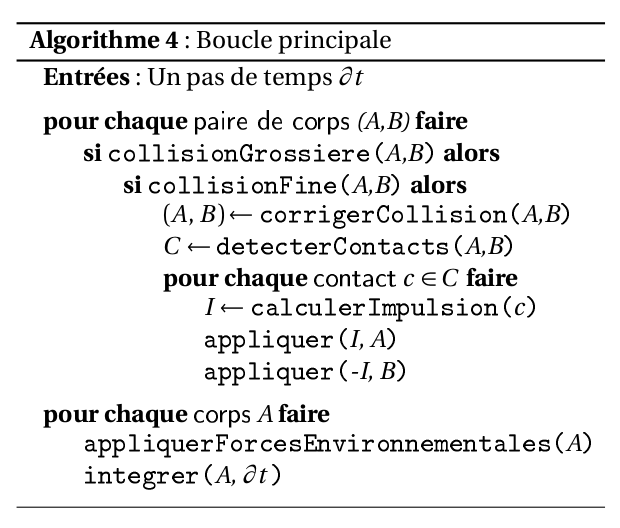
\includegraphics[width=9cm]{images/algo1.png}
  \end{figure}
\end{frame}

\begin{frame}{Défauts de cet algorithme}
  \begin{itemize}
    \item Aucune cohérence temporelle

      \vfill

    \item L'ordre d'intégration des corps change l'issue de la simulation \\

      \vfill

      \begin{figure}
        \begin{tikzpicture}[scale=0.7,transform shape]
  \coordinate (A1) at (0,0);
  \coordinate (A2) at (4.2,0);
  \coordinate (B1) at (5,0);
  \coordinate (B2) at (5,-3);

  \node[
    circle,
    minimum size=1cm,
    draw=bleu,
    thick] at (A1) (a1) {};
  \node[
    circle,
    minimum size=1cm,
    draw=bleu,
    thick,
    dotted] at (A2) (a2) {};
  \draw[->,thick,vert,font=\large] (A1) to node[black,auto] {$+ \deriv t$} (A2);

  \node[
    circle,
    minimum size=1cm,
    draw=rose,
    thick] at (B1) (b1) {};
  \node[
    circle,
    minimum size=1cm,
    draw=rose,
    thick,
    dotted] at (B2) (b2) {};
  \draw[->,thick,vert,font=\large] (B1) to node[black,auto] {$+ \deriv t$} (B2);

\end{tikzpicture}

      \end{figure}
  \end{itemize}
\end{frame}

\begin{frame}{Algorithme principal amélioré}
  \begin{figure}
    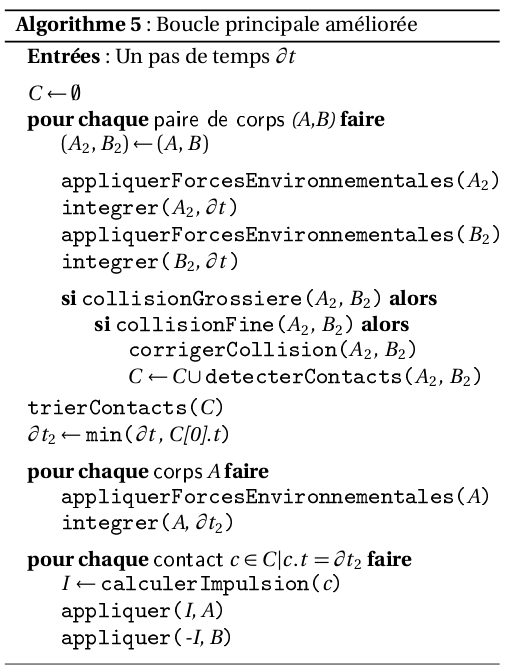
\includegraphics[width=6cm]{images/algo2.png}
  \end{figure}
\end{frame}

\subsection{Démonstrations}

\begin{frame}{Démonstrations}
  \begin{figure}
    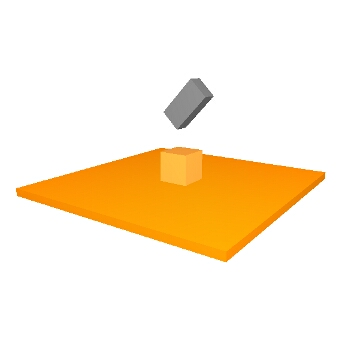
\includegraphics[width=5cm]{images/box.jpg}
    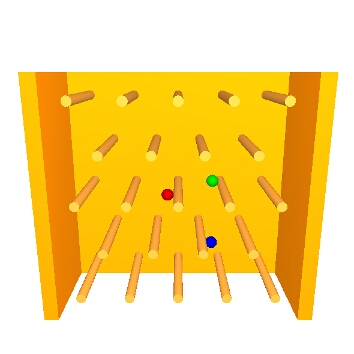
\includegraphics[width=5cm]{images/pachinko.jpg}
  \end{figure}
\end{frame}

\subsection{Perspectives d'évolution}

\begin{frame}{Tunneling}
  \begin{description}
    \item[Problème]
      Les corps se traversent mais aucune collision détectée
  \end{description}

  \vfill

  \begin{overprint}

    \onslide<1>
    \begin{figure}
      \centering
      \begin{tikzpicture}[scale=0.7, transform shape]
  \coordinate (AT1) at (0,0);
\coordinate (AT2) at (8,0);
\coordinate (B) at (6,0);

\draw node[fig,
  circle,
  minimum size=2cm,
  draw=bleu,
  dotted] (a1) at (AT1) {};

\node[fig,
  circle,
  minimum size=2cm,
  draw=bleu] (a2) at (AT2) {};
\node[fig,
  circle,
  minimum size=1cm,
  draw=rose] (b) at (B) {};



  \draw[->,thick,vert] (AT1) to node[black,auto] {$\deriv t$} (AT2);
\end{tikzpicture}

    \end{figure}

    \onslide<2>
    \begin{figure}
      \centering
      \begin{tikzpicture}[scale=0.7, transform shape]
  \coordinate (AT1) at (0,0);
\coordinate (AT2) at (8,0);
\coordinate (B) at (6,0);

\draw node[fig,
  circle,
  minimum size=2cm,
  draw=bleu,
  dotted] (a1) at (AT1) {};

\node[fig,
  circle,
  minimum size=2cm,
  draw=bleu] (a2) at (AT2) {};
\node[fig,
  circle,
  minimum size=1cm,
  draw=rose] (b) at (B) {};



  \path[rayon] (a1.north) -- (a2.north);
  \path[rayon] (a1.west) -- (a2.west);
  \path[rayon] (a1.north west) -- (a2.north west);
  \path[rayon] (a1.south) -- (a2.south);
  \path[rayon] (a1.south west) -- (a2.south west);
\end{tikzpicture}

    \end{figure}
    \vfill
    \begin{description}
    \item[Solution] Lancer de rayons
    \item[+] \'Economique
    \item[--] Peut manquer les plus petits corps
    \end{description}

    \onslide<3>
    \begin{figure}
      \centering
      \begin{tikzpicture}[scale=0.7, transform shape]
  \coordinate (AT1) at (0,0);
\coordinate (AT2) at (8,0);
\coordinate (B) at (6,0);

\draw node[fig,
  circle,
  minimum size=2cm,
  draw=bleu,
  dotted] (a1) at (AT1) {};

\node[fig,
  circle,
  minimum size=2cm,
  draw=bleu] (a2) at (AT2) {};
\node[fig,
  circle,
  minimum size=1cm,
  draw=rose] (b) at (B) {};



  \coordinate (a1n) at ($(a1.north)+(0,0.2)$);
  \coordinate (a2s) at ($(a2.south)+(0,-0.2)$);

  \draw[gris] (a1n) arc (90:270:1.2cm) --
  (a2s) arc (-90:90:1.2cm) --
  (a1n);
\end{tikzpicture}

    \end{figure}
    \vfill
    \begin{description}
    \item[Solution] Boîtes englobant les positions avant/après
    \item[+] Ne manque aucun tunneling
    \item[+] Procédures de base déjà utilisées pour la détection grossière
    \item[--] Certaines trajectoires peu avantageuses (diagonales)
    \end{description}

  \end{overprint}
\end{frame}

\section{Conclusion}

\begin{frame}{Conclusion}
  Différentes perspectives d'évolution :
  \begin{itemize}
    \item Partitionnement de l'espace
    \item Contraintes
    \item Plus de stabilitité (empilement)
  \end{itemize}

  \vfill

  Une voie intéressante : résolution de systèmes linéaires pour les contact de repos.
\end{frame}

\begin{frame}
  \begin{center}
    \Huge{Questions}
  \end{center}
\end{frame}

\end{document}
